%\documentclass[12pt,t]{beamer}
% \documentclass[t]{beamer}
\documentclass[handout]{beamer}\usepackage[]{graphicx}\usepackage[]{color}
%% maxwidth is the original width if it is less than linewidth
%% otherwise use linewidth (to make sure the graphics do not exceed the margin)
\makeatletter
\def\maxwidth{ %
  \ifdim\Gin@nat@width>\linewidth
    \linewidth
  \else
    \Gin@nat@width
  \fi
}
\makeatother

\definecolor{fgcolor}{rgb}{0.345, 0.345, 0.345}
\newcommand{\hlnum}[1]{\textcolor[rgb]{0.686,0.059,0.569}{#1}}%
\newcommand{\hlstr}[1]{\textcolor[rgb]{0.192,0.494,0.8}{#1}}%
\newcommand{\hlcom}[1]{\textcolor[rgb]{0.678,0.584,0.686}{\textit{#1}}}%
\newcommand{\hlopt}[1]{\textcolor[rgb]{0,0,0}{#1}}%
\newcommand{\hlstd}[1]{\textcolor[rgb]{0.345,0.345,0.345}{#1}}%
\newcommand{\hlkwa}[1]{\textcolor[rgb]{0.161,0.373,0.58}{\textbf{#1}}}%
\newcommand{\hlkwb}[1]{\textcolor[rgb]{0.69,0.353,0.396}{#1}}%
\newcommand{\hlkwc}[1]{\textcolor[rgb]{0.333,0.667,0.333}{#1}}%
\newcommand{\hlkwd}[1]{\textcolor[rgb]{0.737,0.353,0.396}{\textbf{#1}}}%
\let\hlipl\hlkwb

\usepackage{framed}
\makeatletter
\newenvironment{kframe}{%
 \def\at@end@of@kframe{}%
 \ifinner\ifhmode%
  \def\at@end@of@kframe{\end{minipage}}%
  \begin{minipage}{\columnwidth}%
 \fi\fi%
 \def\FrameCommand##1{\hskip\@totalleftmargin \hskip-\fboxsep
 \colorbox{shadecolor}{##1}\hskip-\fboxsep
     % There is no \\@totalrightmargin, so:
     \hskip-\linewidth \hskip-\@totalleftmargin \hskip\columnwidth}%
 \MakeFramed {\advance\hsize-\width
   \@totalleftmargin\z@ \linewidth\hsize
   \@setminipage}}%
 {\par\unskip\endMakeFramed%
 \at@end@of@kframe}
\makeatother

\definecolor{shadecolor}{rgb}{.97, .97, .97}
\definecolor{messagecolor}{rgb}{0, 0, 0}
\definecolor{warningcolor}{rgb}{1, 0, 1}
\definecolor{errorcolor}{rgb}{1, 0, 0}
\newenvironment{knitrout}{}{} % an empty environment to be redefined in TeX

\usepackage{alltt}
\usepackage{pgfpages}
\usepackage{pgffor}

% \pgfpagesuselayout{4 on 1}[a4paper,landscape]
% \pagestyle{empty} % descomentar para impresión muy blanca

\usepackage[utf8]{inputenc}
\usepackage[spanish]{babel}
\decimalpoint
\usepackage{verbatim}
\usepackage{hyperref}
%\hypersetup{colorlinks=false,linkbordercolor=red,linkcolor=green,pdfborderstyle={/S/U/W 1}}
%\hypersetup{colorlinks=true,linkbordercolor=red,linkcolor=green,pdfborderstyle={/S/U/W 1}}
\hypersetup{colorlinks=true,linkcolor=blue,pdfborderstyle={/S/U/W 1}}

\usepackage{amsfonts,amssymb,amsmath,amsthm, wasysym}
\usepackage{listings}
%\usepackage[T1]{fontenc}        
\usepackage{pgf}
%\usepackage{epsdice}
\usepackage{pgfpages}
\usepackage{tikz}
\usetikzlibrary{arrows,shapes,plotmarks,backgrounds,trees,positioning}
\usetikzlibrary{decorations.pathmorphing,calc,snakes}
%\usepackage{marvosym}
%
\usetheme[hideothersubsections,left]{Marburg}
%\usetheme[hideothersubsections,left]{Madrid}
%\usetheme[hideothersubsections,left]{Dresden}
%\usetheme{Darmstadt}
\usecolortheme{sidebartab}
\useinnertheme[shadow]{rounded}

% \useoutertheme[footline=empty,subsection=true,compress]{infolines}
% \useoutertheme[footline=empty,subsection=true,compress]{miniframes}
% \usefonttheme{serif}

\setbeamertemplate{caption}[numbered]
%\setbeamertemplate{navigation symbols}{}
\addtobeamertemplate{navigation symbols}{}{%
    \usebeamerfont{footline}%
    \usebeamercolor[fg]{footline}%
    \hspace{1em}%
    \insertframenumber/\inserttotalframenumber
    
    \setbeamercolor{footline}{fg=blue}
\setbeamerfont{footline}{series=\bfseries}
}

\newcommand{\red}[1]{\textcolor{red}{#1}}
\newcommand{\green}[1]{\textcolor{green}{#1}}
\newcommand{\blue}[1]{\textcolor{blue}{#1}}
\newcommand{\gray}[1]{\textcolor{gray}{#1}}
\renewcommand{\emph}[1]{{\color{red}#1}}

%\newtheorem{theorem}



\setbeamertemplate{frametitle}
{\begin{centering}
\medskip
\color{blue}
\textbf{\insertframetitle}
\medskip
\end{centering}
}
\usecolortheme{rose}
\usecolortheme{dolphin}
\mode<presentation>


\newcommand{\CC}{\mathbb{C}}
\newcommand{\RR}{\mathbb{R}}
\newcommand{\ZZ}{\mathbb{Z}}
\newcommand{\NN}{\mathbb{N}}
\newcommand{\KK}{\mathbb{K}}
\newcommand{\MM}{\mathcal{M}}
%\newcommand{\dbinom}{\displaystyle\binom}

\newcommand{\limn}{{\displaystyle lim_{n\to\infty}}}

%\renewcommand{\lim}{\displaystyle \mathrm{lim}}
\renewcommand{\leq}{\leqslant}
\renewcommand{\geq}{\geqslant}
\def\tendeix{{\displaystyle\mathop{\longrightarrow}_{\scriptscriptstyle
n\to\infty}}}

\newcommand{\matriu}[1]{\left(\begin{matrix} #1 \end{matrix}\right)}

% \newcommand{\qed}{\hbox{}\nobreak\hfill\vrule width 1.4mm height 1.4mm depth 0mm
%     \par \goodbreak \smallskip}
%
% %

\theoremstyle{plain}
\newtheorem{teorema}{Teorema}
%\newtheorem{prop}{Proposición}
\newtheorem{prop}{Propiedades}
\newtheorem{cor}{Corolario}
\theoremstyle{definition}
\newtheorem{ejemplo}{Ejemplo}
\newtheorem{definicion}{Definición}
\newtheorem{obs}{Observación}

\newcounter{seccions}
\newcommand{\seccio}[1]{\addtocounter{seccions}{1}
\medskip\par\noindent\textbf{\theseccions.
#1}\smallskip\par }

\newcommand{\EM}{\Omega}
\newcommand{\PP}{\mathcal{P}}

\title[\red{Matemáticas III GINF}]{}
\author[]{R. Alberich}
\date{}
\IfFileExists{upquote.sty}{\usepackage{upquote}}{}
\begin{document}
\beamertemplatedotitem

\lstset{backgroundcolor=\color{green!50}}
\lstset{breaklines=true}
\lstset{basicstyle=\ttfamily}


\section{Variables aleatorias continuas notables.}

\begin{frame}
\vfill
\begin{center}
\gray{\LARGE Distribuciones notables III. Distribuciones continuas }
\end{center}
\vfill
\end{frame}
%\section{Algunas distribuciones continuas}


\begin{frame}
\begin{itemize}
\item Para acabar este tema veremos algunas distribuciones continua notables.
\item En concreto veremos las distribuciones uniforme, normal o gaussiana y exponencial.
\item Al final del tema y de forma \emph{OPCIONAL} se estudian las   aproximaciones de la distribución binomial y Poisson por la normal.
\end{itemize}
\end{frame}

\subsection{Distribución  uniforme}

\begin{frame}[fragile]
\frametitle{Distribución uniforme}
Una v.a. continua $X$ tiene \emph{distribución uniforme}
sobre el intervalo real
$(a,b)$ ($a<b$), y lo indicaremos con \emph{$U(a,b)$}, si  su función de densidad es
 $$
 f_X(x)=
 \left\{\begin{array}{ll}
\dfrac{1}{b-a} & \mbox{si } a<x<b\\[2ex] 0  & \mbox{si $x\leq a$ o $x\geq b$}
\end{array}
\right. $$ 
Una variable $U(a,b)$ modela la elección de  un punto del intervalo $(a,b)$ de manera ``\textsl{equiprobable}'' (mejor isodensa)
\medskip

Con {\tt R}, es \texttt{unif}

\end{frame}


\begin{frame} 
\frametitle{Distribución uniforme}
 $U(1,5):\quad f_X(x)=
 \left\{\begin{array}{ll}
\dfrac{1}{4} & \mbox{si } 1<x<5\\[2ex] 0  & \mbox{si $x\leq 1$ o $x\geq 5$}
\end{array}
\right. $

\begin{center}
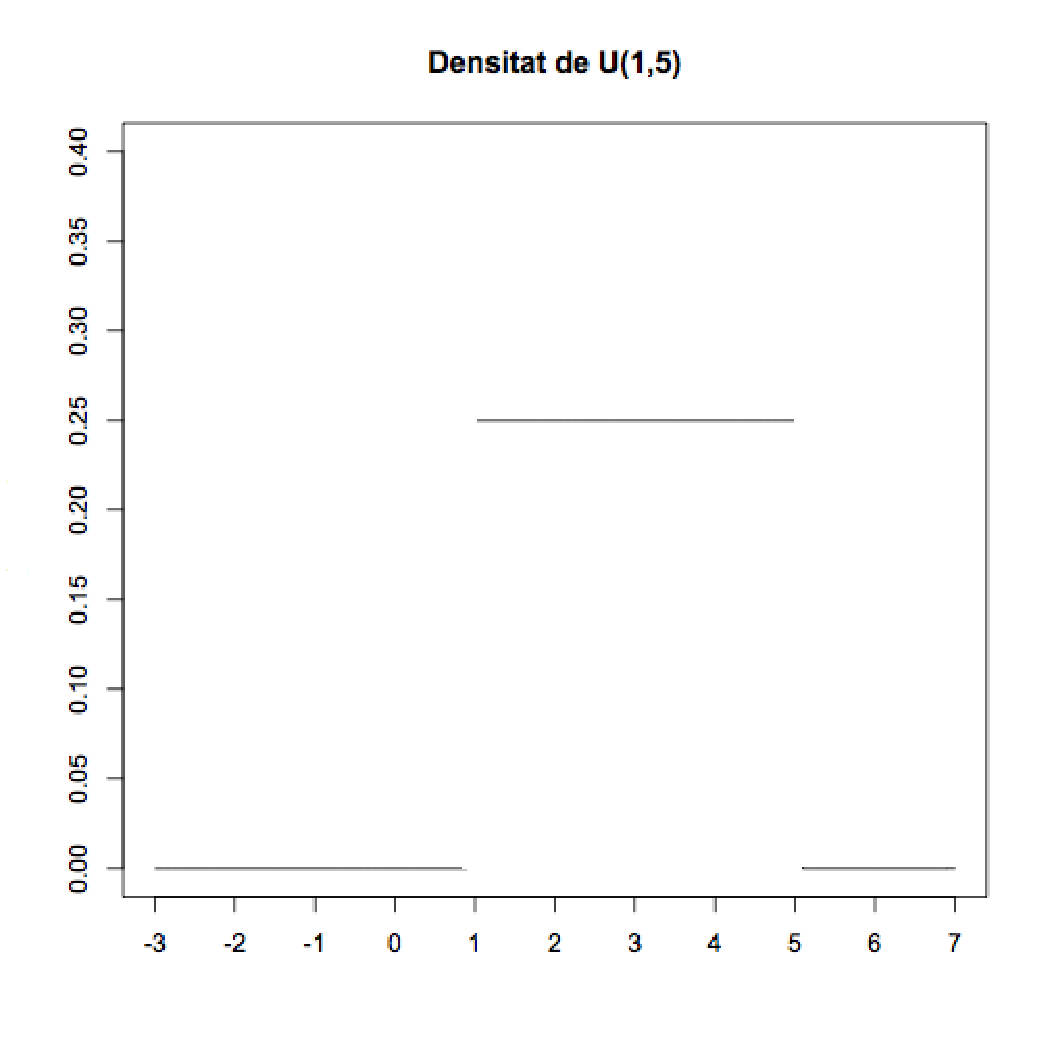
\includegraphics[width=0.6\linewidth]{dunif15}
\end{center}



\end{frame}


 
\begin{frame} 
\frametitle{Distribución uniforme}
\vspace*{-1ex}

Integrando, la función de distribución obtenemos:
$$
F_X(x)=\left\{\begin{array}{ll} 0  & \mbox{si } x\leq a\\
\dfrac{x-a}{b-a} & \mbox{si } a<x<b\\ 1  & \mbox{si } b\leq x
\end{array}
\right. 
$$
\vspace*{-3ex}

\begin{center}
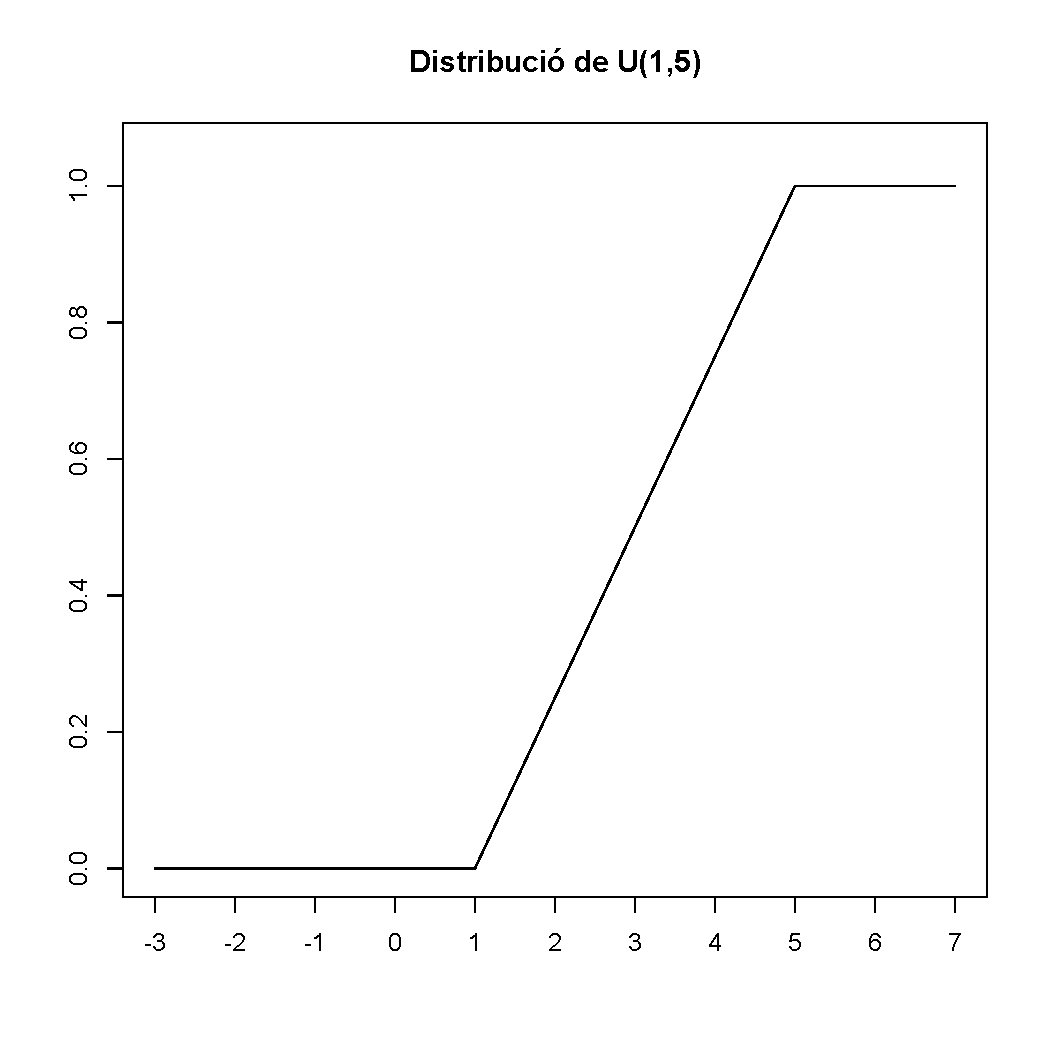
\includegraphics[width=0.625\linewidth]{punif15}
\end{center}



\end{frame}


\begin{frame}
\frametitle{Resumen v.a. uniforme en el intervalo $(a,b)$}
\vspace*{-2ex}


\scriptsize
\setlength{\tabcolsep}{1pt}
\begin{table}
\centering
\begin{tabular}{|rl|}
\hline 
\multicolumn{2}{|c|}{$X\equiv U(a,b)$.}\\ 
\hline
\hline 
$D_X=$&  $(a,b)$ \\\hline 
$f_x(x)=$& 
$f_X(x)=\left\{\begin{array}{ll}
\dfrac{1}{b-a} & \mbox{si } a<x<b\\ 0  & \mbox{ si $x\leq a$ o $x\geq b$}
\end{array} \right.$
\\ \hline 
$F_X(x)=P(X\leq X)=$ &  $F_X(x)=\left\{\begin{array}{ll} 0 & \mbox{ si } x\leq a\\
          \dfrac{x-a}{b-a} & \mbox{ si } a\leq x\leq b\\
          1 & \mbox{ si } b\leq x\end{array}\right.$\\
          \hline 
$E(X)=$ &  $\frac{a+b}{2}$ \\
$Var(X)=$ & $\frac{(b-a)^2}{12}$\\
\hline
\end{tabular}
\end{table}
\normalsize
\end{frame}




\begin{frame}
\frametitle{Esperanza y varianza}
\vspace*{-2ex}

Sea $X$ una v.a. $U(a,b)$
\vspace*{-3ex}

\begin{eqnarray*}
\red{E(X)} &\hspace*{-1ex}= & \hspace*{-2ex}\int_{-\infty}^{+\infty} \hspace*{-3ex}x \cdot f_X(x)\, dx=\int_{a}^{b} \hspace*{-1ex}x \frac{1}{b-a}\, dx \\ &\hspace*{-2ex}= & \hspace*{-2ex}
\Big[\frac{x^2}{2(b-a)}\Big]_{a}^{b}=\red{\frac{b+a}{2}} \\[2ex] 
E(X^2)& \hspace*{-1ex}=  & \hspace*{-2ex} \int_{-\infty}^{+\infty} \hspace*{-3ex} x^2\cdot f_X(x)\, dx=\int_{a}^{b}  \hspace*{-1ex}x^2 \frac{1}{b-a}\, dx \\ &\hspace*{-2ex}= & \hspace*{-2ex}\Big[\frac{x^3}{3(b-a)}\Big]_{a}^{b} =\frac{b^3-a^3}{3(b-a)} = \frac{b^2+ab+a^2}{3} \\ 
\red{Var(X)} & \hspace*{-1ex}= & \hspace*{-1ex} E(X^2)-(E(X))^2=\frac{b^2+ab+a^2}{3}-\left(\frac{b+a}{2}\right)^2\\ & \hspace*{-1ex}= & \hspace*{-1ex} \red{\frac{(b-a)^2}{12}}
\end{eqnarray*}
\end{frame}

%\begin{frame}
%\frametitle{Exemple}
%
%Tenim una espècie de plantes angiospermes, les flors de la qual no demostren cap preferència en la seva orientació, y per tant cada flor admet totes les orientacions amb la mateixa probabilitat\bigskip
%
%
%Si mesuram l'orientació en graus, amb el 0 a l'est y en sentit antihorari, podem considerar que la v.a. $X$ que dóna aquesta orientació és $U(0,360)$
%\medskip
%
%Densitat: $f_X(x)=\left\{\begin{array}{ll}
%\dfrac{1}{360} & \mbox{si } 0<x<360\\[2ex] 0  & \mbox{ si $x\leq 0$ o $x\geq 360$}
%\end{array} \right.$
%
%\end{frame}
%
%\begin{frame}
%\frametitle{Exemple}
%
%
%\blue{Quina és la probabilitat que una flor estigui orientada exactament a nord ($90^{\mathrm{o}}$)?}
%\medskip
%\pause
%
%$\displaystyle P(X=90)=0$
%\bigskip
%\pause
%
%
%\blue{Quina és la probabilitat que una flor estigui orientada a nord, amb un error de menys de $5^{\mathrm{o}}$?}
%\medskip
%\pause
%
%$\displaystyle P(85<X<95)=\int_{85}^{95}\frac{1}{360}\,dt=\Big[\frac{t}{360}\Big]_{85}^{95}=\frac{10}{360}=\frac{1}{36}$
%\bigskip
%\pause
%
%\blue{Quina és la desviació típica de les orientacions de les flors?}
%\medskip
%\pause
%
%$\displaystyle \sigma=\sqrt{\frac{360^2}{12}}=\frac{360}{\sqrt{12}}\approx 103.9^{\mathrm{o}}$
%
%
%
%\end{frame}
%



\subsection{Distribución  normal}

\begin{frame}
\frametitle{Distribución normal}
Una v.a. $X$ sigue una \emph{ley normal} o \emph{gaussiana} de
parámetros $\mu$ y $\sigma$, y lo indicaremos con \red{$N(\mu,\sigma)$}, cuando tiene función de densidad $$
f_{X}(x)=\frac{1}{\sqrt{2\pi}\sigma} e^{{-(x-\mu)^2}/{(2\sigma^{2})}} \mbox{
para todo} x\in \RR
$$
\bigskip

Cuando $\mu=0$ y $\sigma=1$, diremos que la v.a. normal es \emph{estándar}, y la indicaremos usualmente con  $Z$
$$
f_{Z}(x)=\frac{1}{\sqrt{2\pi}} e^{ -x^2/2} \mbox{
para todo  } x\in \RR
$$

Con  R, es \texttt{norm}
\end{frame}


\begin{frame}
\frametitle{Resumen de distribución normal o gaussiana.}
\vspace*{-2ex}
\scriptsize
\setlength{\tabcolsep}{2pt}
\begin{table}
\centering
\begin{tabular}{|rl|}
\hline 
\multicolumn{2}{|c|}{$X\equiv N(\mu,\sigma)$.}\\ 
\hline
\hline 
$D_X=$&  $(-\infty,+\infty)$ \\\hline 
$f_x(x)=$& 
$\frac{1}{\sqrt{2\pi}\sigma} e^{{-(x-\mu)^2}/{(2\sigma^{2})}}.$\\ \hline 
$F_X(x)=P(X\leq X)=$ &  No tiene expresión, tablas o función de R\\
\hline 
$E(X)=$ & $\mu$\\
$Var(X)=$ & $\sigma^2$\\
\hline
\end{tabular}
\end{table}
\normalsize
\end{frame}




\begin{frame} 
\frametitle{Distribución normal}
La gráfica de $f_X$ es la conocida \emph{campana de Gauss}

%\begin{center}
%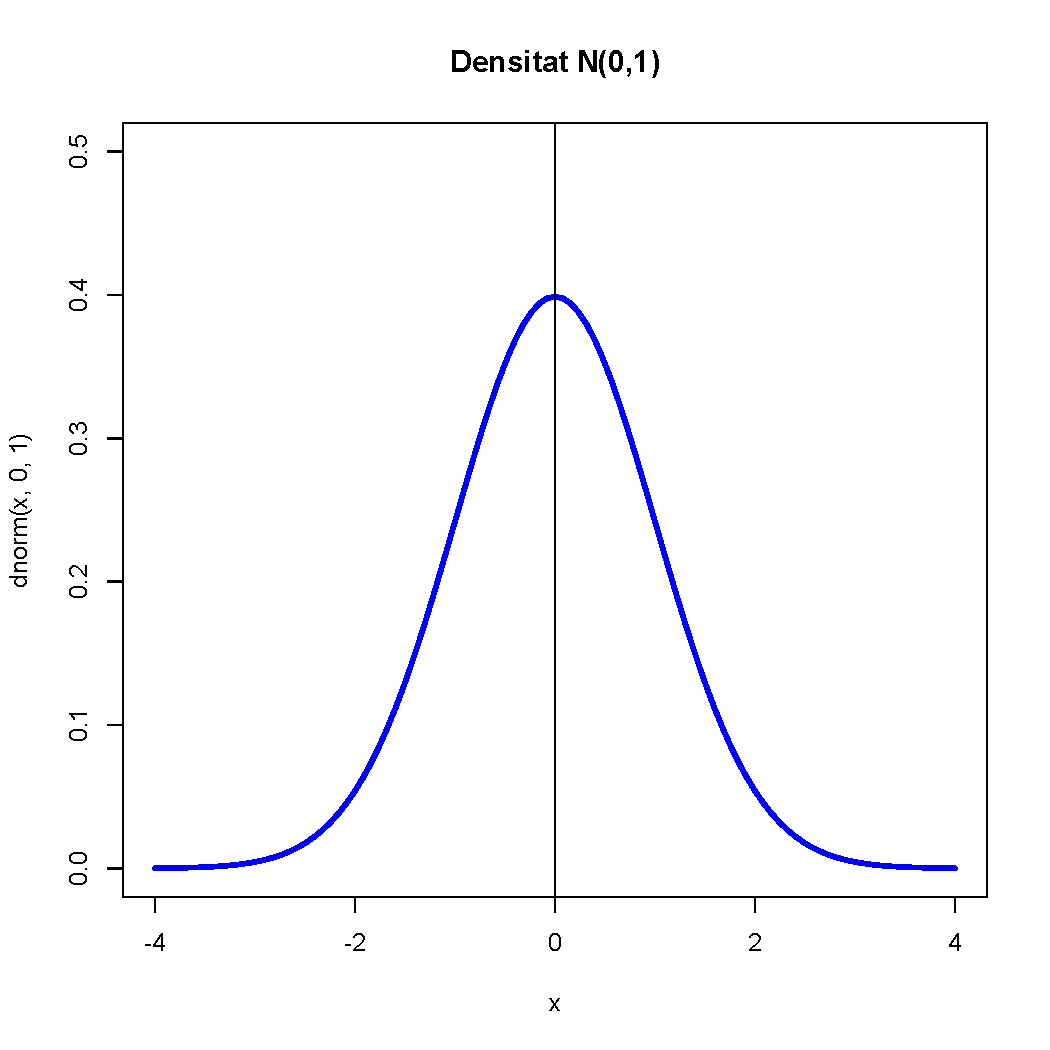
\includegraphics[width=0.8\linewidth]{dnorm01}
%\end{center}

\begin{knitrout}
\definecolor{shadecolor}{rgb}{0.969, 0.969, 0.969}\color{fgcolor}
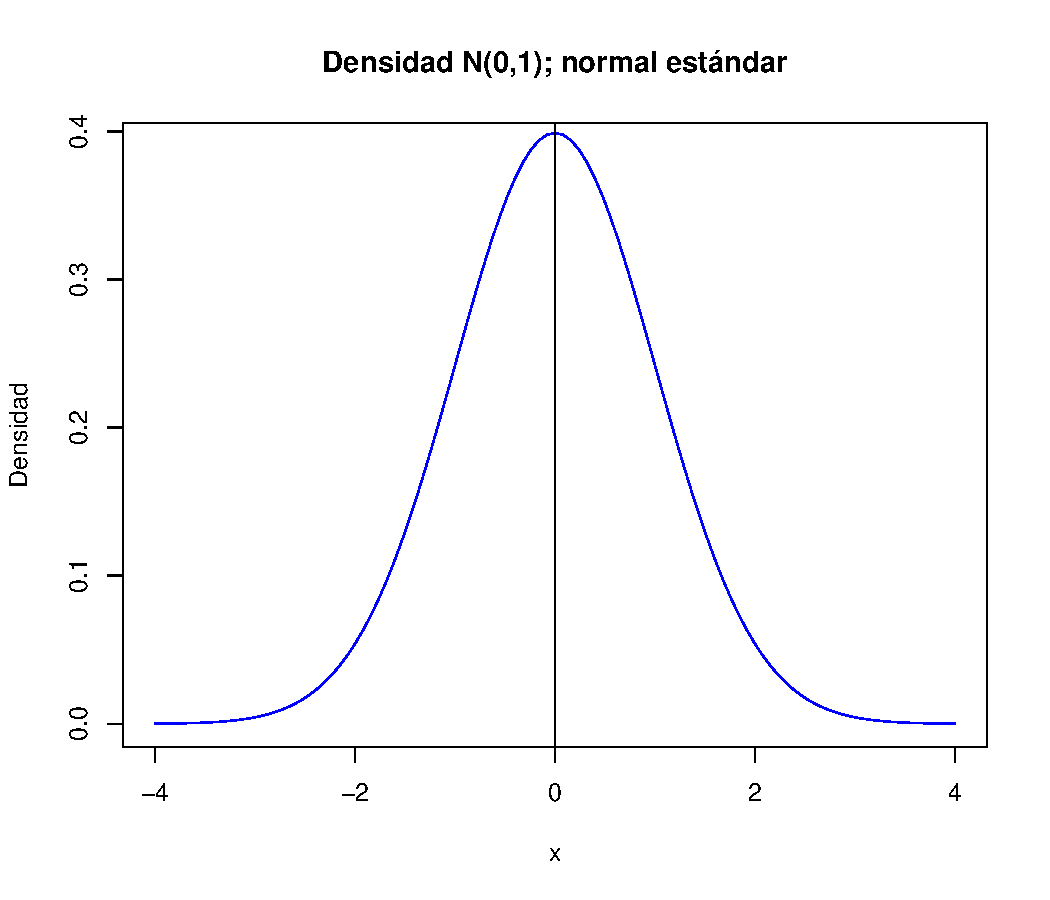
\includegraphics[width=\maxwidth]{figure/unnamed-chunk-1-1} 

\end{knitrout}




\end{frame}


\begin{frame} 
\frametitle{Distribución normal}



La distribución normal es una de les más importantes y utilizadas en estadística, porque aproxima muy bien muchos fenómenos:
\medskip

\begin{itemize}
\item Alturas, inteligencia,\ldots
\item Calificaciones, aciertos, errores de medida, \ldots
\end{itemize}

Además, 
\begin{itemize}
\item Muchas variables aleatorias consistentes en  tomar una muestra de $N$ elementos y calcular alguna cosa (por ejemplo, la media) tienen distribución aproximadamente normal cuando $N$ es grande, aunque  que las distribuciones de los elementos individuales no lo sean
\end{itemize}


\end{frame}


\begin{frame}
\frametitle{Propiedades} 
\vspace*{-1ex}

Sea $X$ una v.a. $N(\mu,\sigma)$
\medskip

\begin{itemize}
\item $f_X$ es simétrica respecto de $x=\mu$:
$$
f_{X}(\mu-x)=f_{X}(\mu+x)
$$
y  tiene  el máximo en $x=\mu$
\medskip

En particular, si $Z$ es una $N(0,1)$, entonces
$f_{Z}(-x)=f_{Z}(x)$, y $f_Z$ toma el valor máximo en  $x=0$
\end{itemize}
\vspace*{-5ex}

\begin{center}
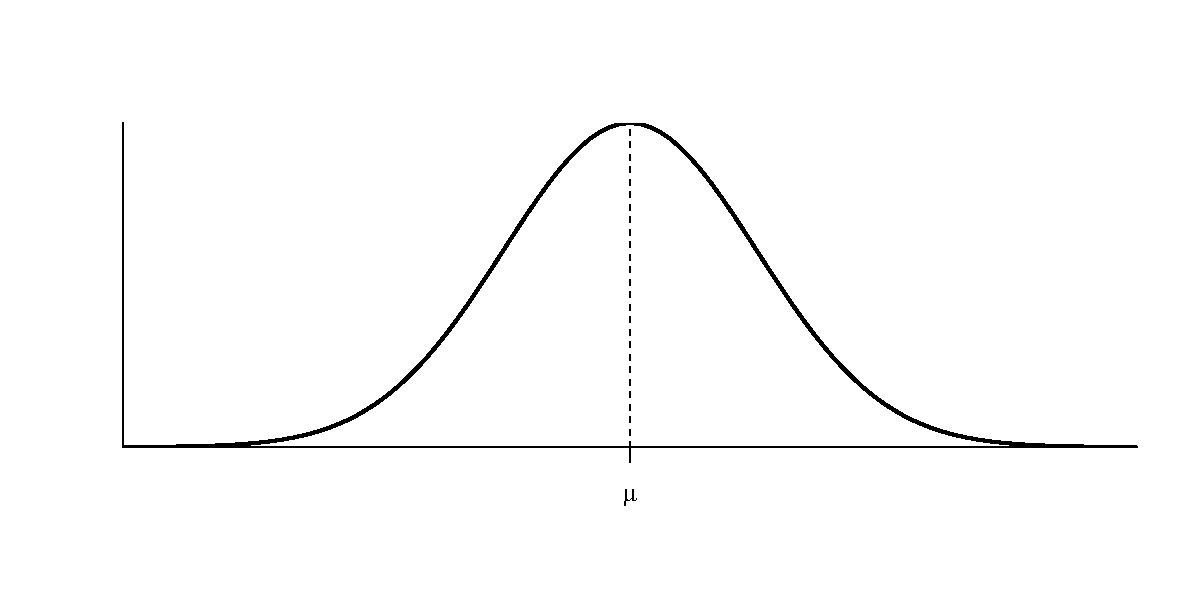
\includegraphics[width=\linewidth]{simn}
\end{center}
\end{frame}

%
%\begin{frame}
%\frametitle{Propietats} 
%
%Recordem que $P(X\leq x)=F_X(x)$ és l'àrea compresa entre $f_X$, l'eix $y=0$ y la recta vertical a $x$
%\begin{center}
%\includegraphics[width=\linewidth]{undernorm}
%\end{center}
%\end{frame}
%

\begin{frame}
\frametitle{Propiedades} 
\begin{itemize}
\item Esta simetría hace que las áreas  de la izquierda de $\mu-x$ y de la  derecha de $\mu+x$ sean iguales

\begin{center}
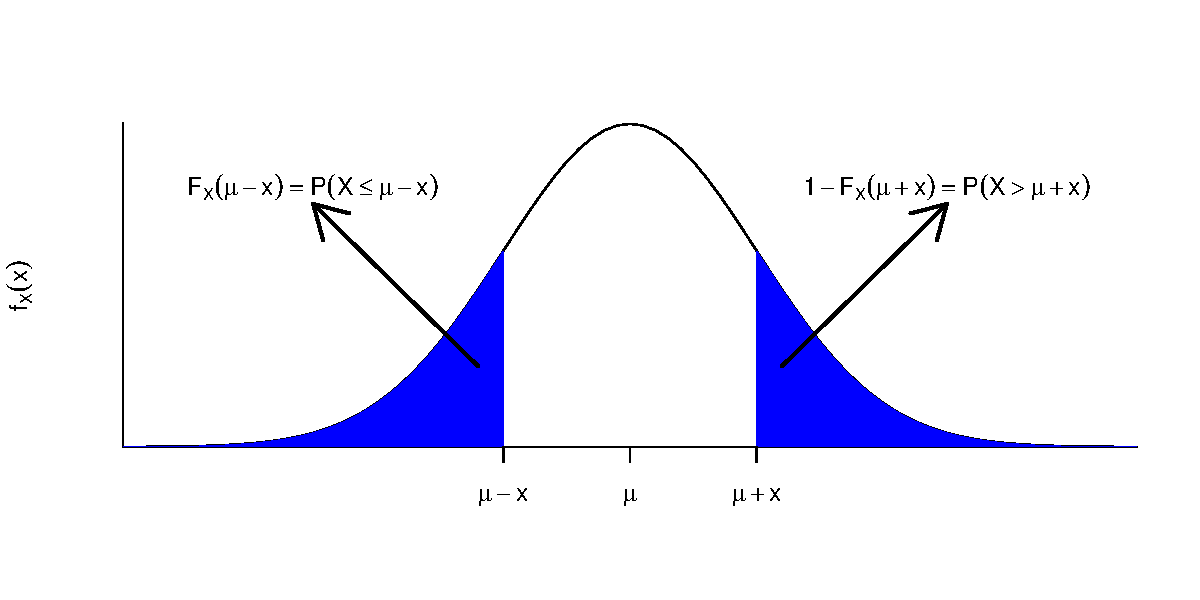
\includegraphics[width=\linewidth]{simnorm1}
\end{center}
\vspace*{-1.5cm}

$$
\begin{array}{rl}
\red{F_{X}(\mu-x)} & =P(X\leq \mu-x)\\ &
=P(X\geq \mu+x) \red{{} =1-F_{X}(\mu+x)}
\end{array}
$$
\end{itemize}
\end{frame}


\begin{frame}
\frametitle{Propiedades} 
\begin{itemize}
\item En una $N(0,1)$, esta simetría hace iguales  las áreas  a la izquierda de  $-z$ y a la derecha de $z$
\begin{center}
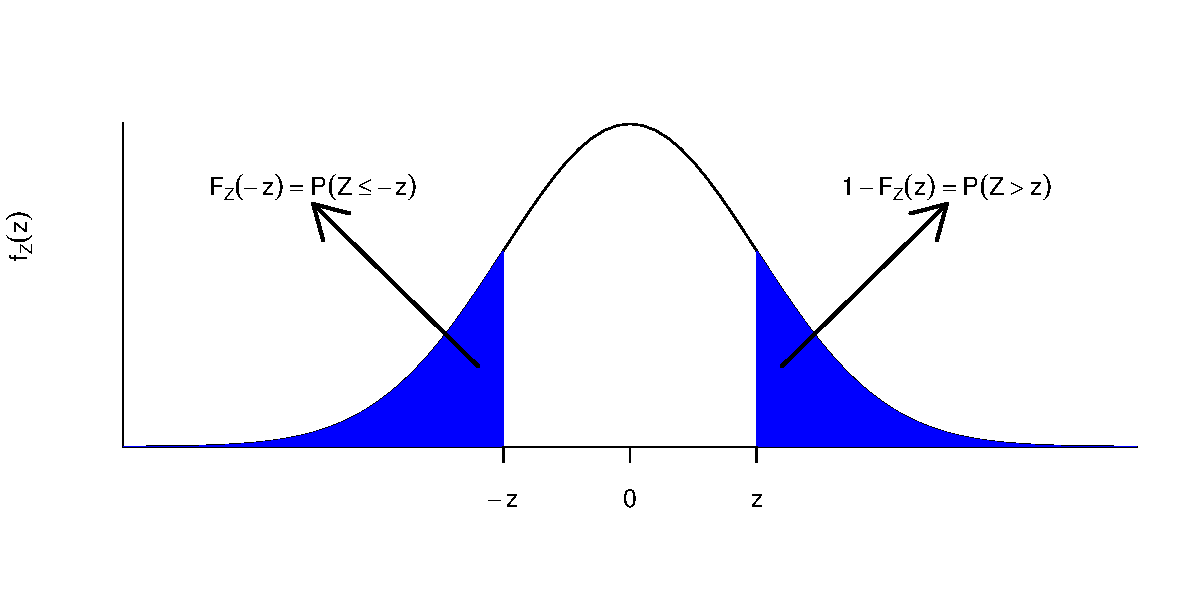
\includegraphics[width=\linewidth]{simnorm2}
\end{center}
\vspace*{-1cm}

$$
\red{F_{Z}(-z)}=P(Z\leq -z)=P(Z\geq  z)\red{{} =1-F_{Z}(z)}
$$
\end{itemize}
\end{frame}

\begin{frame}
\frametitle{Propiedades} 
Sea $X$ una v.a. $N(\mu,\sigma)$
\medskip

\begin{itemize}


\item$E(X)=\mu$ 
\medskip

\item$Var(X)=\sigma^2$ 
\medskip

\item  Su desviación típica es $\sigma$
\end{itemize}
\bigskip

En particular, si $Z$ es una normal estándar, $E(Z)=0$ y $Var(Z)=1$.
\end{frame}



\begin{frame}
\frametitle{Distribución normal}

Aumentar la $\mu$ desplaza a la derecha el máximo de la densidad, y con el toda la curva
\begin{center}
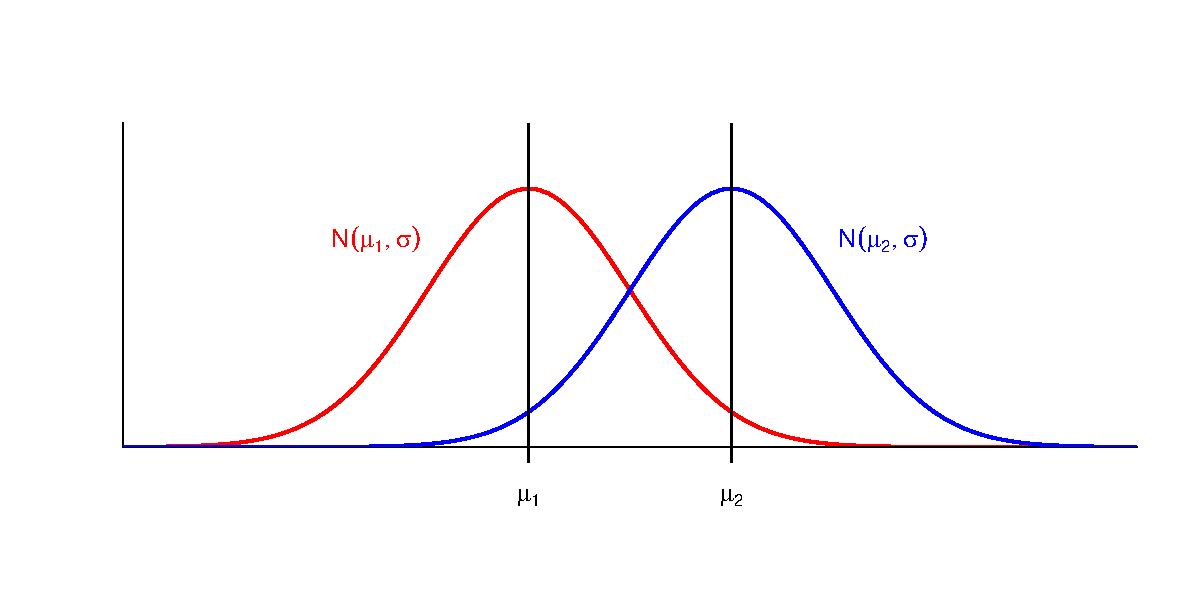
\includegraphics[width=\linewidth]{mu1mu2}

$\mu_1<\mu_2$
\end{center}
\end{frame}




\begin{frame}
\frametitle{Distribución normal}

Augmentar la $\sigma$ achata la curva: al aumentar la varianza, los valores se alejan más del valor medio.
\begin{center}
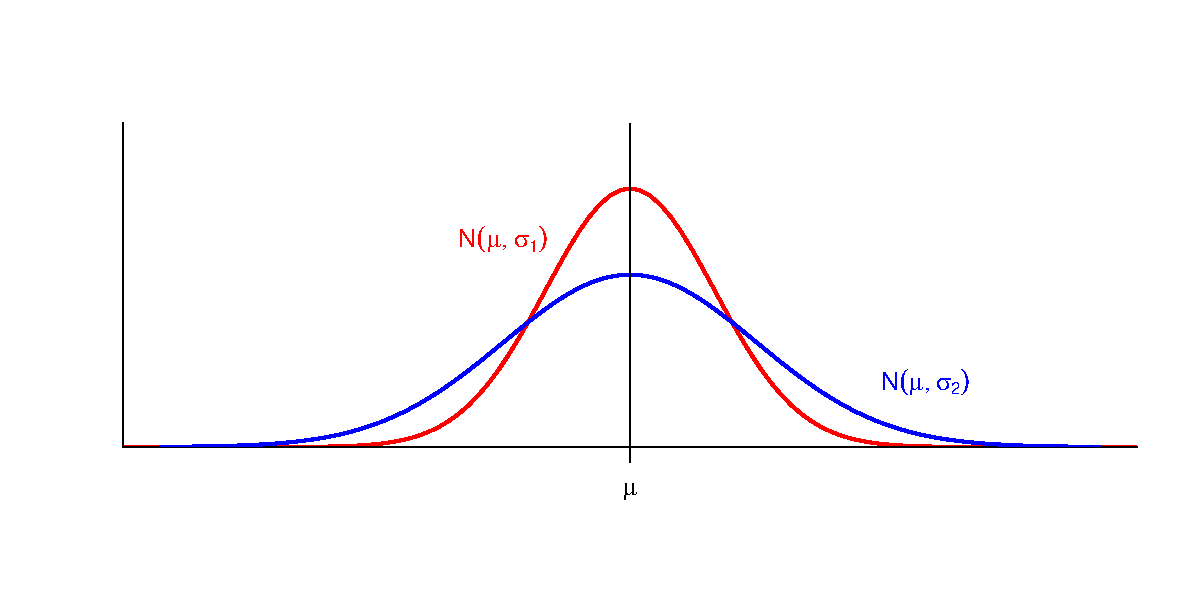
\includegraphics[width=\linewidth]{sigma1sigma2}

$\sigma_1<\sigma_2$
\end{center}
\end{frame}




\begin{frame}
\frametitle{Distribución normal}

El efecto combinado es
\begin{center}
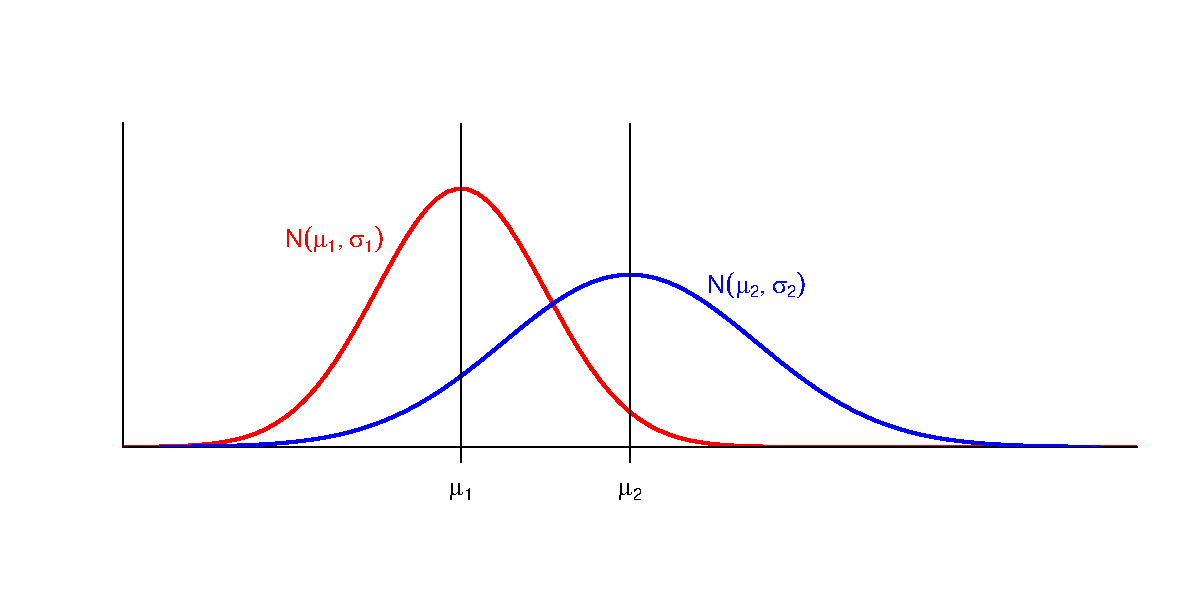
\includegraphics[width=\linewidth]{musigma}

$\mu_1<\mu_2,\ \sigma_1<\sigma_2$
\end{center}
\end{frame}




\begin{frame}
\frametitle{Estandarización  o tipificación de una v.a.\ normal}

\begin{teorema}
Si $X$ es una v.a. $N(\mu,\sigma)$, entonces
$Z=\dfrac{X-\mu}{\sigma}$
es $N(0,1)$.
\end{teorema}

Las probabilidades de una normal estándar $Z$ determinan las de cualquier $X$  con distribución  $N(\mu,\sigma)$:
$$
\begin{array}{rl}
\red{P(X\leq x)} & \displaystyle \hspace*{-1ex} =P\Big(\frac{X-\mu}{\sigma}\leq \frac{x-\mu}{\sigma}\Big)\red{=P\Big(Z\leq \frac{x-\mu}{\sigma}\Big)}\\[1ex]
\red{P(y\leq X\leq x)} & \displaystyle \hspace*{-1ex} =P\Big( \frac{y-\mu}{\sigma}\leq \frac{X-\mu}{\sigma}\leq \frac{x-\mu}{\sigma}\Big)\\[1ex] & \displaystyle \hspace*{-1ex} \red{=P\Big(\frac{y-\mu}{\sigma}\leq Z\leq \frac{x-\mu}{\sigma}\Big)}
\end{array}
$$
\end{frame}


\begin{frame}
\frametitle{Cálculo de probabilidades}
\vspace*{-2ex}

$F_Z$ no tiene expresión conocida. La podemos calcular con  R (\texttt{pnorm}), o, de forma manual, con tablas.
Las tablas para calcular $F_Z$ están en  el espacio Moodle de la asignatura.
\vspace*{-2ex}

\begin{center}
\hspace*{-0.4cm}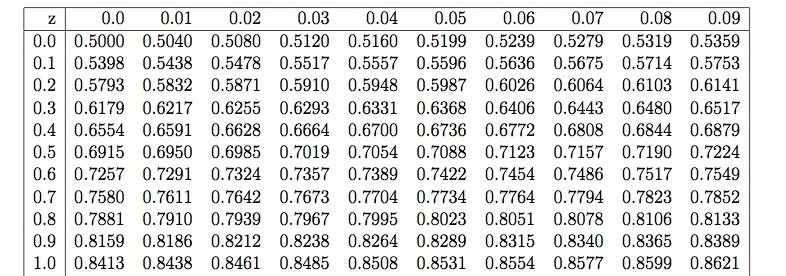
\includegraphics[width=1.1\linewidth]{tabla.jpg}
\end{center}
\pause

{\small $F_Z(0.75)=0.7734,\pause\ F_Z(1.02)=0.8461,\pause\ F_Z(0.06)=\pause 0.5239$\\[1ex]
\pause

$F_Z(-0.75)=1-F_Z(0.75)=0.2266,\pause\ F_Z(-0.88)=\pause 0.1894$

}
\end{frame}


\begin{frame}
\frametitle{Cálculo de probabilidades}
\vspace*{-1cm}

\begin{center}
\hspace*{-0.2cm}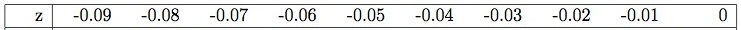
\includegraphics[width=1.06\linewidth]{taula4.jpg}
$$
\vdots
$$
\hspace*{-0.4cm}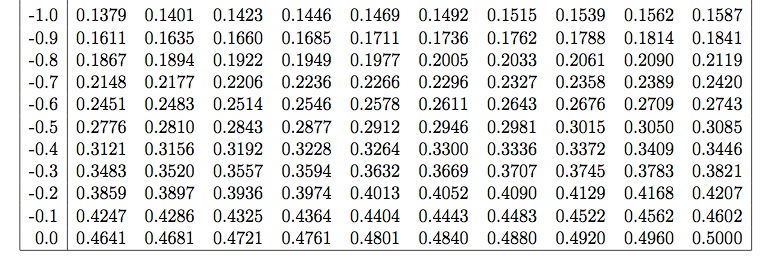
\includegraphics[width=1.1\linewidth]{tabla2.jpg}
\end{center}

{\small 
$F_Z(-0.75)= 0.2266,\ F_Z(-0.88)= 0.1894$

}
\end{frame}



\begin{frame}
\frametitle{Cálculo de probabilidades}
\vspace*{-1cm}

\begin{center}
\hspace*{-0.4cm}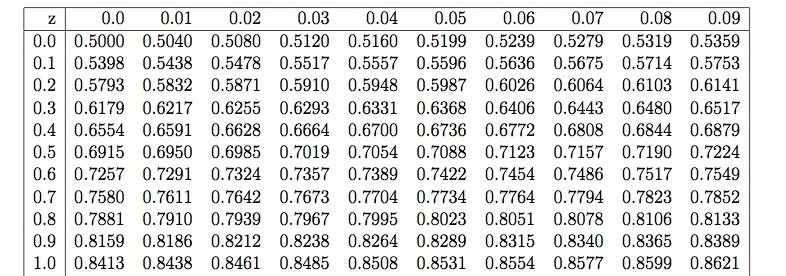
\includegraphics[width=1.1\linewidth]{tabla.jpg}
\end{center}
$$
\begin{array}{rl}
P(0.25<Z<0.75) & =P(Z<0.75)-P(Z<0.25)\\ & =0.7734-0.5987=0.1747\\[2ex]\pause
P(-0.3<Z<0.3) & =\pause P(Z<0.3)-P(Z<-0.3)\\ & =P(Z<0.3)-1+P(Z<0.3)\\ & =2P(Z<0.3)-1=0.2358
\end{array}
$$
\end{frame}


%\begin{frame}
%
%\frametitle{Exemple} 
%Sea $Z$ una variable normal estándar. Utilizando las tablas de la distribución
%normal estándar calcular las siguientes probabilidades:
%\begin{enumerate}[a)]
%\item $P(0< Z < 3.99)=F_Z(3.99)-F_Z(0)\approx 1-0.5=0.5$. 
%\item $P(-3.99\leq Z \leq 3.99)=F_{Z}(3.99)-F_{Z}(-3.99)\approx 1.$
%\item $P(-3\leq Z \leq 3)=F_{Z}(3)-F_{Z}(-3)= 0.9987-0.0013=0.9974$.
%\item $P(Z\leq -2)=F_Z(-2)=0.0228$.
%\item $P( Z \leq 2)=F_{Z}(2)=0.9772$.
%\item $P( Z \geq 2)=1-P(Z<2)=1-F_{Z}(2)=0.0228$.
%\item $P( Z \geq -2)=1-P(Z< -2)=1-F_{Z}(-2)=1-(1-F_Z(2))=F_Z(2)$.
%\item Dado $\delta>0$, $P(-\delta\leq Z \leq
%\delta)=F_{Z}(\delta)-F_{Z}(-\delta)=F_Z(\delta)-(1-F_Z(\delta))=2\cdot 
%F_Z(\delta)-1$.
%\item Utilizando la igualdad anterior
%$P(-2\leq Z \leq 2)=2\cdot  F_Z(2)-1=2 \cdot 0.9772-1=0.9544$.
%\end{enumerate}
%
%\end{frame}


\begin{frame}
\frametitle{Cálculo de cuantiles}

Les tablas  también  se pueden utilizar para ``calcular'' cuantiles (con R, \texttt{qnorm}).
\medskip

Si queremos saber el valor de $z$ tal que $P(Z\leq z)=q$, buscamos en la tabla la entrada $q$ (o la más próxima)  y  miramos a que $z$ corresponde.
\vspace*{-3ex}

\begin{center}
\hspace*{-0.4cm}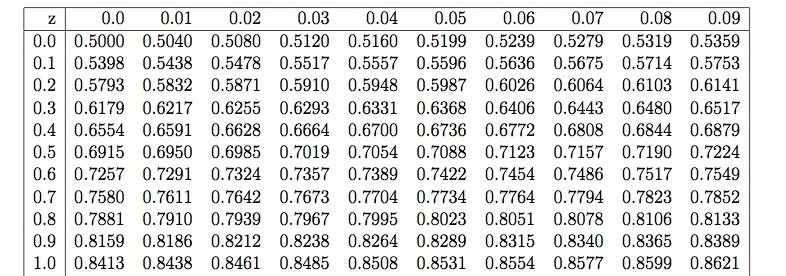
\includegraphics[width=1.1\linewidth]{tabla.jpg}
\end{center}
\vspace*{-2ex}

¿Cuál es el valor de  $z$ tal que $P(Z\leq z)=0.7357$? $z=0.63$


\end{frame}

\begin{frame}[fragile]
\frametitle{Cálculo de  cuantiles}
\vspace*{-1cm}


\begin{center}
\hspace*{-0.4cm}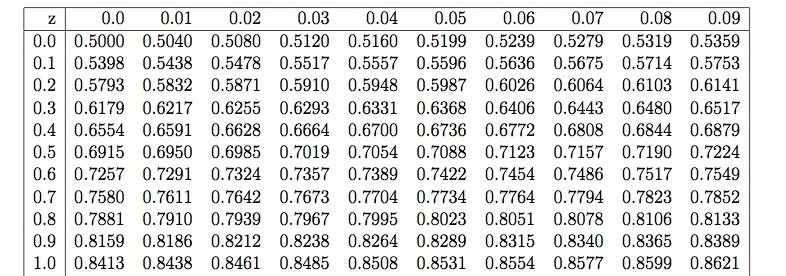
\includegraphics[width=1.1\linewidth]{tabla.jpg}
\end{center}
\vspace*{-2ex}

¿Cuál es el valor de  $z$ tal que $P(Z\leq z)=0.8357$?\\ \pause Entre 0.97 y 0.98
\begin{knitrout}
\definecolor{shadecolor}{rgb}{0.969, 0.969, 0.969}\color{fgcolor}\begin{kframe}
\begin{alltt}
\hlkwd{qnorm}\hlstd{(}\hlnum{0.8357}\hlstd{)}
\end{alltt}
\begin{verbatim}
## [1] 0.9769377
\end{verbatim}
\end{kframe}
\end{knitrout}
\end{frame}


\begin{frame}
\frametitle{Con las  normales no estándar\ldots}
\vspace*{-1cm}

\begin{center}
\hspace*{-0.4cm}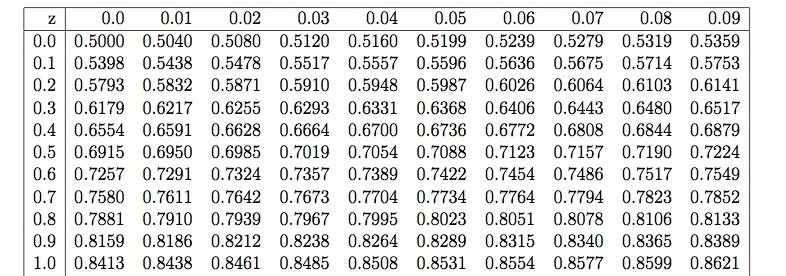
\includegraphics[width=1.1\linewidth]{tabla.jpg}
\end{center}

Sea $X$ una v.a. $N(1,2)$. ¿Qué vale $P(X\leq 2)$?
$$
P(X\leq 2)=P\Big(Z\leq\frac{2-1}{2}=0.5\Big)=0.6915
$$

\end{frame}

\begin{frame}
\frametitle{Con  las normales no estándar\ldots}
\vspace*{-1cm}

\begin{center}
\hspace*{-0.4cm}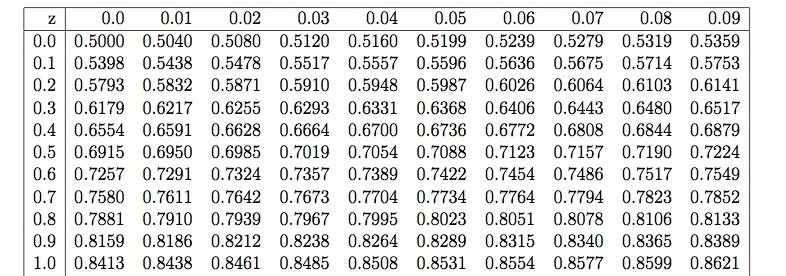
\includegraphics[width=1.1\linewidth]{tabla.jpg}
\end{center}

Sea $X$ una v.a. $N(1,2)$. ¿Para qué   valor de $x$ se tiene que  $P(X\leq x)=0.7939$?

$$
\begin{array}{l}
0.7939=P(X\leq x)=P\Big(Z\leq\dfrac{x-1}{2}\Big)\\[1ex]\qquad\qquad\qquad\qquad \Rightarrow \dfrac{x-1}{2}=0.82
\Rightarrow x=2.64
\end{array}
$$

\end{frame}

\begin{frame}
\frametitle{Con las normales no estándar\ldots}
\vspace*{-1cm}

\begin{center}
\hspace*{-0.4cm}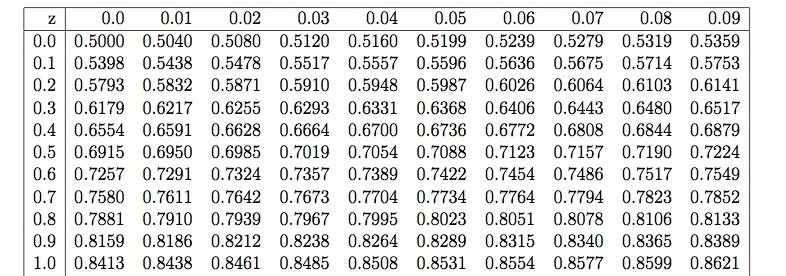
\includegraphics[width=1.1\linewidth]{tabla.jpg}
\end{center}

Sea $X$ una v.a. $N(0.5,1.5)$. \medskip

¿Qué vale $P(X\leq 1.5)$? \medskip

¿Para qué  $x$ se tiene  que $P(X\leq x)=0.834$?



\end{frame}




\subsection{Distribución exponencial}

\begin{frame}[fragile]
\frametitle{Distribución exponencial}
Una v.a. continua $X$ tiene \emph{distribución exponencial} de  parámetro $\lambda$,  y lo  indicaremos con   \emph{$Exp(\lambda)$}, si su  función de densidad es
 $$
 f_X(x)=
 \left\{\begin{array}{ll}
0 & \mbox{si } x\leq 0\\[2ex] \lambda e^{-\lambda x}  & \mbox{si $x>0$}
\end{array}
\right. $$ 

Efectivamente esta función es densidad
$$
\int_0^\infty  \lambda e^{-\lambda t}\,dt=\lim_{x\to\infty}\Big[-e^{-\lambda t}\Big]_0^x=\lim_{x\to\infty}-e^{-\lambda x}+1=1
$$

Con  R es \texttt{exp}
%\begin{verbatim}
%> dexp(3,2) #exponencial de  parámetro 2
%[1] 0.004957504
%\end{verbatim}


\end{frame}

\begin{frame} 
\frametitle{Distribución exponencial}

La distribución exponencial es el equivalente continuo de la distribución geométrica discreta en el sentido de carecer de memoria
\medskip

Si $X$ es una v.a. que mide el tiempo entre dos ocurrencias de un determinado acontecimiento,
y  el tiempo  que pueda tardar en pasar el acontecimiento es independiente del que llevemos  esperando hasta ahora, entonces $X$ es exponencial.
\medskip

\begin{itemize}
\item Tiempo que tarda una partícula radioactiva en  desintegrarse

\item Tiempo en  que espera un enfermo en la cola  de un servicio de urgencias
\end{itemize}

\end{frame}

\begin{frame} 
\frametitle{Distribución exponencial}

\begin{teorema}
Si tenemos un proceso de Poisson de  parámetro $\lambda$ por unidad  de tiempo, el tiempo  que pasa entre dos acontecimientos consecutivos es una v.a. $Exp(\lambda)$
\end{teorema}

Si sabemos que la v.a. $X_t$ que da el numero de acontecimientos en el intervalo de  $]0,t]$ es  $Po(\lambda t)$
\medskip

Consideremos  la v.a. $T$ que da el tiempo transcurrido entre dos sentenciosamente consecutivos.
$$
\begin{array}{rl}
P(T>t) & = P(\mbox{0  acontecimientos en el intervalo }]0,t])\\
 & =P(X_t=0)=\dfrac{(\lambda t)^0}{0!} e^{-\lambda t}=e^{-\lambda t}
\end{array}
$$

\end{frame}

\begin{frame} 
\frametitle{Distribución exponencial}

Por tanto
$$
F_T(t) = \left\{
\begin{array}{ll}
\hspace*{-1ex}
0 & \mbox{si $t\leq 0$}\\
\hspace*{-1ex}
P(T\leq t)\!=\!1-P(T>t)\!=\! 1-e^{-\lambda t} & \mbox{si $t> 0$}
\end{array}\right.
$$
Derivando
$$
f_{T}(t)=F_T'(t)=
\left\{\begin{array}{ll}
          0 & \mbox{ si } t\leq 0\\
        \lambda e^{-\lambda t} & \mbox{ si }  t>0
         \end{array}\right.
$$

Es $Exp(\lambda)$

\end{frame}


\begin{frame}
\frametitle{Resumen de distribución exponencial}
\vspace*{-2ex}
\scriptsize
\setlength{\tabcolsep}{2pt}
\begin{table}
\centering
\begin{tabular}{|rl|}
\hline 
\multicolumn{2}{|c|}{$X\equiv Exp(\lambda)$.}\\ 
\hline
\hline 
$D_X=$&  $(0,+\infty)$ \\\hline 
$f_x(x)=$& 
$\left\{\begin{array}{ll}
0 & \mbox{si } x\leq 0\\ \lambda e^{-\lambda x}  & \mbox{ si $x>0$}
\end{array} \right.$\\ \hline 
$F_X(x)=P(X\leq X)=$ &  
$\left\{
\begin{array}{ll} 0 & \mbox{si $x\leq 0$}\\
  1-e^{-\lambda x} & \mbox{si $x> 0$}
  \end{array}\right.
$\\
\hline 
$E(X)= \frac{1}{\lambda}$  &  $Var(X)=\frac{1}{\lambda^2}$\\
\hline
\end{tabular}
\end{table}
\normalsize
\end{frame}


 
\begin{frame}
    \frametitle{Propiedad de la falta de memoria}


\begin{teorema}
Si $X$  es una v.a. $Exp(\lambda)$,  entonces 
$$
P(X> s+t|X> s)=P(X>t)\mbox{ para  todo $s,t>0$}
$$
\end{teorema}
\medskip

La probabilidad de que, a partir de un cierto momento, tengamos que esperar más de una cantidad de tiempo $t$   para que  pase  el acontecimiento  que cuenta  $X$, no depende del tiempo que llevemos esperando.
 \end{frame}



\begin{frame}
\frametitle{Ejemplo}

Supongamos que en un determinada infección por una bacteria el número de bacterias que se reproducen por división  en un intervalo de tiempo es un proceso de Poisson, y que de media se divide una bacteria cada 2 minutos.\medskip

Si $X_t$ es el número de bacterias  que se dividen en $t$ minutos, $X_t$ es $Po(\lambda t)$, con  $\lambda$ el número medio bacterias que se dividen en un minuto: $\lambda=\frac{1}{2}$.\medskip


Sea $T$ el tempo entre dos divisiones  bacterias  consecutivas. Por lo que hemos visto, $T$ es  $Exp(\frac{1}{2})$.
 \end{frame}



\begin{frame}
\frametitle{Ejemplo}

\blue{Acabamos de observar la  división de una bacteria. ¿Cuál  es la probabilidad de que tengamos que esperar más de 5 minutos  hasta la siguiente división?}
\pause
$$
\begin{array}{rl}
P(T>5) & =1-P(T\leq 5)=1-F_T(5)\\ & =1-(1-e^{-\frac{1}{2}\cdot 5}) =
e^{-\frac{5}{2}}=0.0821
\end{array}
$$
\pause

\blue{Acabamos de observar la  división de una bacteria. ¿Cuál  es la probabilidad de que tengamos que  esperar entre 5 y 10  minuto hasta la próxima división?}
\pause
$$
\begin{array}{rl}
P(5<T<10)  & =P(T<10)-P(T<5)\\ &=F_T(10)-F_T(5)\\ & =(1-e^{-\frac{1}{2}\cdot 10})-(1-e^{-\frac{1}{2}\cdot 5})\\ & =e^{-\frac{5}{2}}-e^{-5}
\end{array}
$$



\end{frame}



\begin{frame}
\frametitle{Ejemplo}

\blue{¿Cuál es el valor esperado y  la desviación típica  del tiempo que transcurre entre dos divisiones sucesivas?}
\medskip

La esperanza es
$$
E(T)=\frac{1}{\lambda}=\frac{1}{\frac{1}{2}}=2
$$

La desviación típica es
$$
\sigma_T=\sqrt{Var(T)}=\sqrt{\frac{1}{\lambda^2}}=\frac{1}{\lambda}=2
$$


\end{frame}



 
\subsection{(OPCIONAL) Aproximaciones de la binomial y la Poisson por la normal.}
 
\begin{frame}
\frametitle{(OPCIONAL)Aproximación de una binomial por una normal}
\vspace*{-1ex}

Sea  $X$ una v.a. $B(n,p)$, de manera  que $E(X)=n\cdot p$  y
$Var(X)=n\cdot p\cdot q$ (donde $q=1-p$)
\medskip

Si $n$ es grande y $p$ no esta cerca de  0 o 1, entonces  $X$ es aproximadamente $N(np,\sqrt{npq})$
\vspace*{-1ex}

% \begin{center}
% 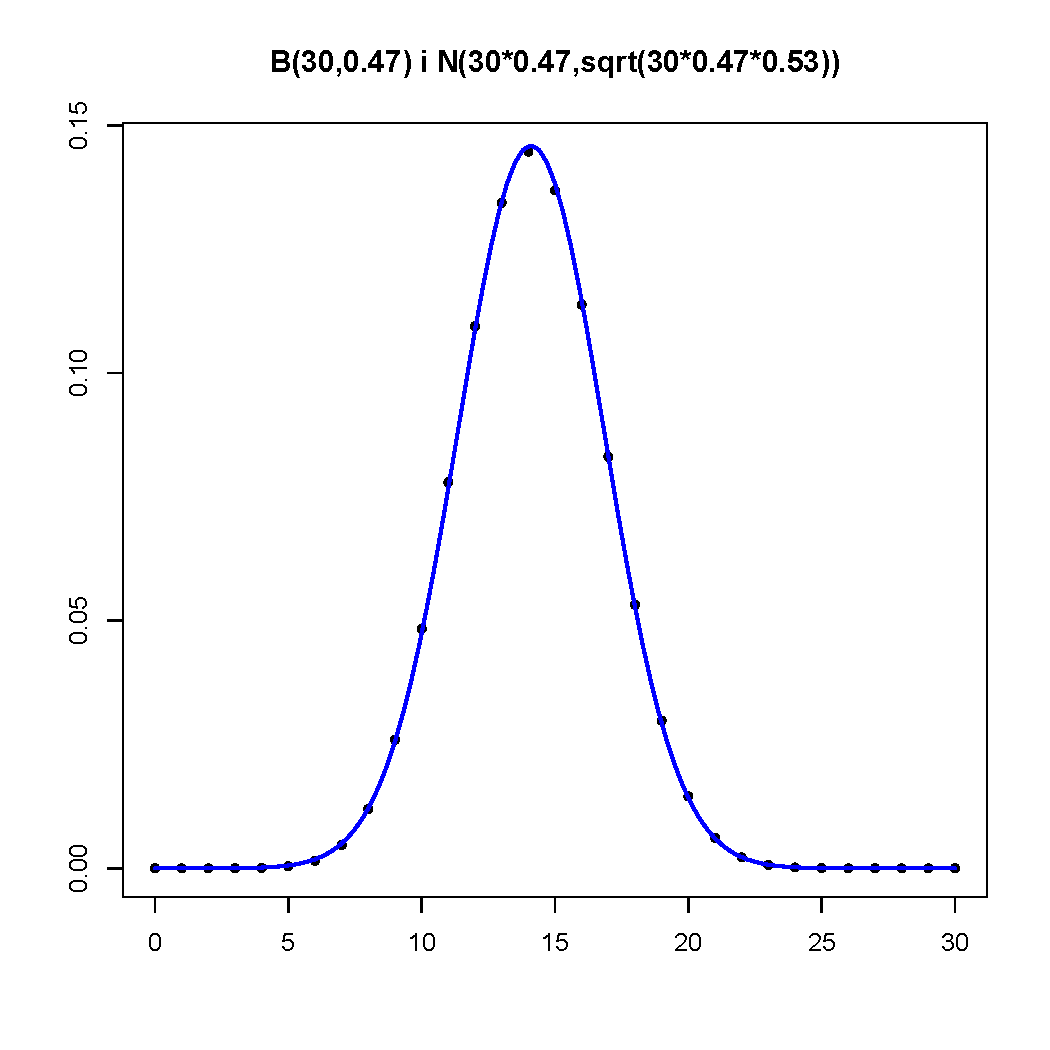
\includegraphics[width=0.58\linewidth]{normvsbin}
% \end{center}
\begin{knitrout}
\definecolor{shadecolor}{rgb}{0.969, 0.969, 0.969}\color{fgcolor}
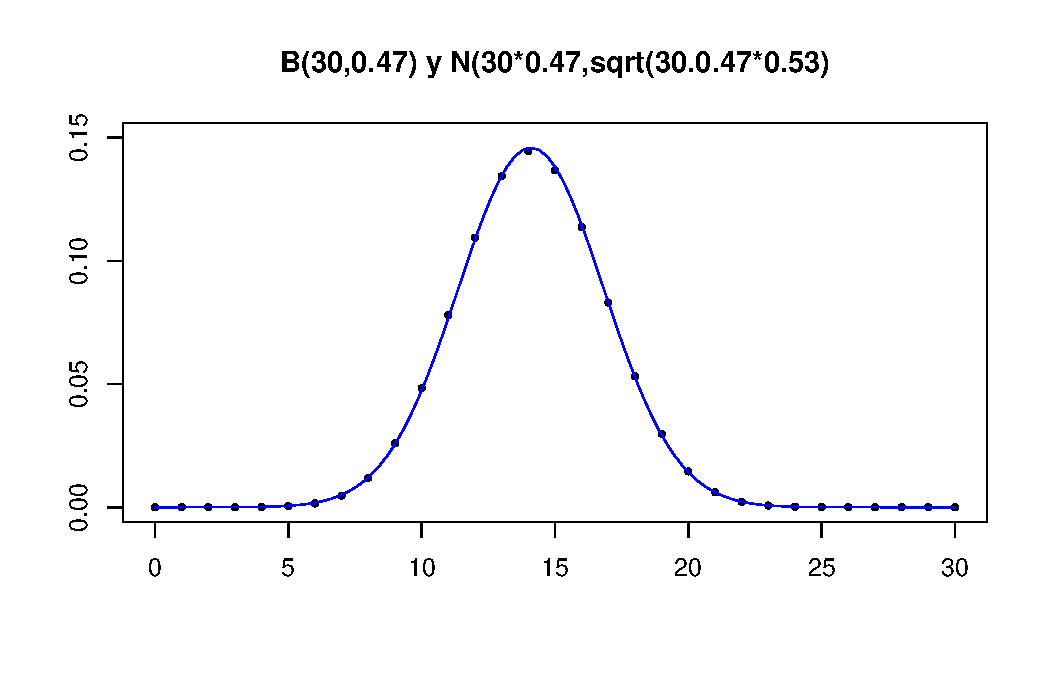
\includegraphics[width=\maxwidth]{figure/unnamed-chunk-3-1} 

\end{knitrout}
\end{frame}

\begin{frame}
\frametitle{(OPCIONAL)Aproximación de una binomial por una normal}
\vspace*{-2ex}

\begin{teorema}
Sea  $X$ una v.a. $B(n,p)$, con $n$ grande y $p$ que no está cerca de 0 o 1. Sea $Y$ una v.a. $N(n\cdot p,\sqrt{n\cdot p\cdot q})$. 

Entonces 
$$
P(X=k)\approx  P\left(k-0.5\leq Y\leq k+0.5\right)
$$
\end{teorema}
De la suma $\pm 0.5$ para corregir el efecto que tiene aproximar una v.a. discreta por una continua se la denomina \emph{corrección de continuidad de Fisher}.
\medskip

Hay diversas heurísticas  para decidir qué quiere decir ``$n$ grande y $p$ no cerca de 0 o 1''. Por ejemplo: $$n\geq 20, n\cdot p\geq 10\mbox{ y }n\cdot (1-p)\geq 10$$

\end{frame}

\begin{frame}[fragile]
\frametitle{(OPCIONAL)Aproximación de una binomial por una normal}
\vspace*{-1ex}

Sea $X\sim B(30,0.47)$: $\mu\!=\!30\!\cdot\! 0.47$ y $\sigma\!=\!\sqrt{30\!\cdot\! 0.47\!\cdot\! 0.53}$
%{\footnotesize \begin{verbatim}
%> dbinom(13,30,0.47)
%[1] 0.134361
%> PY=function(x){pnorm(x,30*0.47,sqrt(30*0.47*0.53))}
%> PY(13.5)-PY(12.5)
%[1] 0.1339606
%\end{verbatim}
\begin{knitrout}
\definecolor{shadecolor}{rgb}{0.969, 0.969, 0.969}\color{fgcolor}\begin{kframe}
\begin{alltt}
\hlkwd{dbinom}\hlstd{(}\hlnum{13}\hlstd{,}\hlnum{30}\hlstd{,}\hlnum{0.47}\hlstd{)}
\end{alltt}
\begin{verbatim}
## [1] 0.134361
\end{verbatim}
\begin{alltt}
\hlstd{PY}\hlkwb{=}\hlkwa{function}\hlstd{(}\hlkwc{x}\hlstd{)\{}\hlkwd{pnorm}\hlstd{(x,}\hlnum{30}\hlopt{*}\hlnum{0.47}\hlstd{,}\hlkwd{sqrt}\hlstd{(}\hlnum{30}\hlopt{*}\hlnum{0.47}\hlopt{*}\hlnum{0.53}\hlstd{))\}}
\hlkwd{PY}\hlstd{(}\hlnum{13.5}\hlstd{)}\hlopt{-}\hlkwd{PY}\hlstd{(}\hlnum{12.5}\hlstd{)}
\end{alltt}
\begin{verbatim}
## [1] 0.1339606
\end{verbatim}
\end{kframe}
\end{knitrout}


\vspace*{-5ex}

\begin{center}
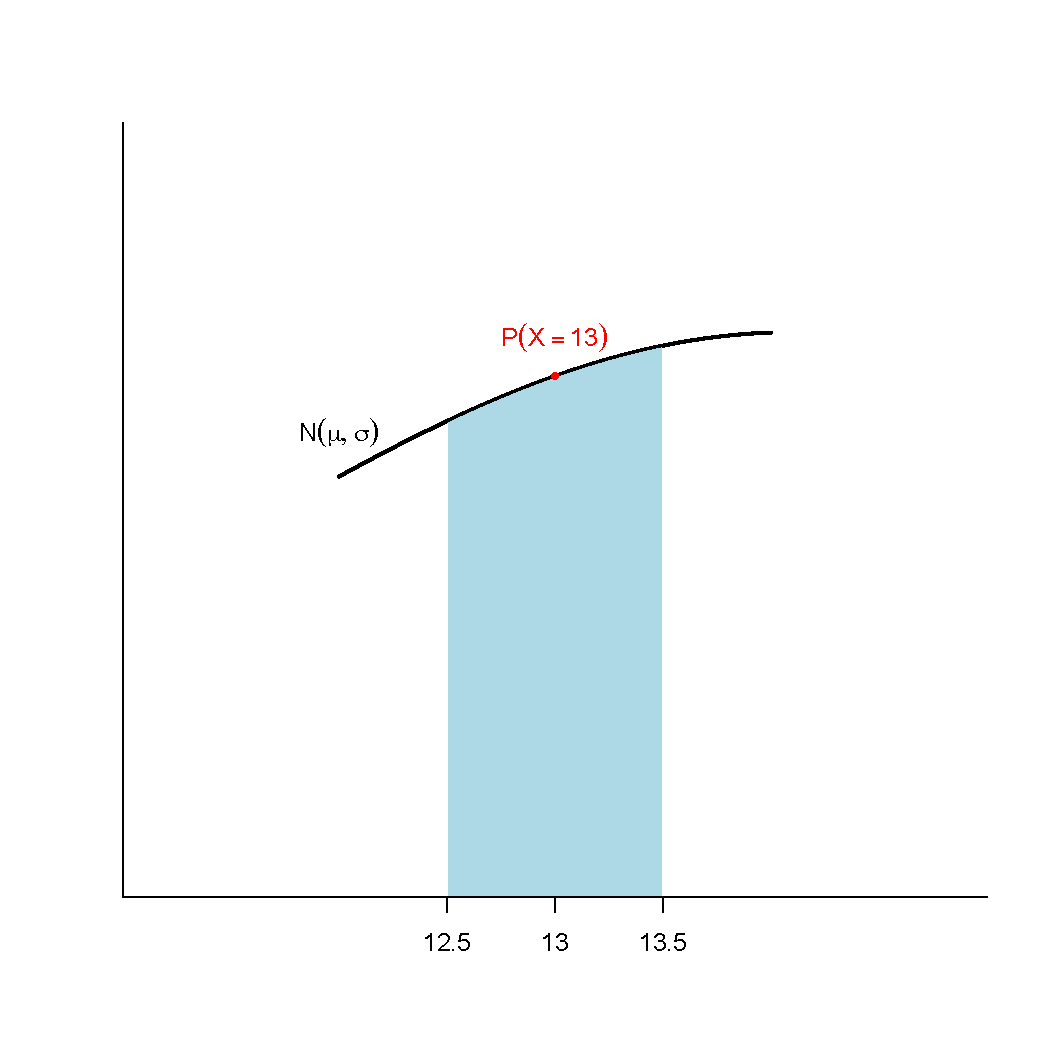
\includegraphics[width=0.4\linewidth]{binomvsnorm1}
\end{center}



\end{frame}




\begin{frame}
\frametitle{(OPCIONAL)Aproximación de una binomial por una normal}
\vspace*{-2ex}

Si $X$ es una v.a. $B(n,p)$ con $n$ grande y $p$ que no  este cerca de  0  ni de  1,
$$
\frac{X-E(X)}{\sqrt{Var(X)}}=\frac{X-np}{\sqrt{npq}}
$$
se aproxima por  una normal estándar $Z$:
$$
P(X=k) \approx P\left(\frac{k-0.5-np}{\sqrt{npq}}\leq Z \leq \frac{k+0.5-np}{\sqrt{npq}}\right)
$$


\end{frame}









\begin{frame}
\frametitle{(OPCIONAL)Aproximación de una binomial por una normal}

Si $X$ es una v.a. $B(n,p)$ con  $n$ gran y $p$ que no esté cerca cde 0 ni de 1 , y $Z$ es una v.a. normal estándar:



$$
\begin{array}{l}
P(X\leq k)  \displaystyle\approx P\left(Z \leq
\frac{{k+0.5-np}}{\sqrt{npq}}\right)\\[3ex]
P(X\geq k)  \displaystyle\approx P\left(
\frac{{k-0.5-np}}{\sqrt{npq}}\leq Z\right)\\[3ex]
P(a\leq X\leq b) \displaystyle\approx
P\left(\frac{a-0.5-np}{\sqrt{npq}}\leq Z \leq
\frac{b+0.5-np}{\sqrt{npq}}\right)
\end{array}
$$
\end{frame}




\begin{frame}[fragile]
\frametitle{Ejemplo}
\blue{Lanzamos 100 veces una moneda con probabilidad de cara $\frac{1}{2}$.
Probabilidad de sacar  40 y 49 caras?}
\bigskip

 $X$=número de caras en 100 lanzamientos de una moneda
 \medskip
 
$X$  es $B(100,0.5)$
 \medskip
 
 
 
 Nos piden $P(40\leq X\leq 49)$
 \medskip

\begin{knitrout}
\definecolor{shadecolor}{rgb}{0.969, 0.969, 0.969}\color{fgcolor}\begin{kframe}
\begin{alltt}
\hlkwd{pbinom}\hlstd{(}\hlnum{49}\hlstd{,}\hlnum{100}\hlstd{,}\hlnum{0.5}\hlstd{)}\hlopt{-}\hlkwd{pbinom}\hlstd{(}\hlnum{39}\hlstd{,}\hlnum{100}\hlstd{,}\hlnum{0.5}\hlstd{)}
\end{alltt}
\begin{verbatim}
## [1] 0.4426053
\end{verbatim}
\end{kframe}
\end{knitrout}

\end{frame}


\begin{frame}
\frametitle{Ejemplo}
\vspace*{-1ex}

Y si no tenemos a mano  {\tt R}? Podemos emplear la tabla de la distribución $N(0,1)$:\medskip

$X\sim B(100,0.5)\Rightarrow E(X)=n\cdot p=50,\ \sigma_{X}=\sqrt{npq}=5$
\medskip

$Z=\dfrac{X-50}{5}\sim N(0,1)$

$$
\begin{array}{l}
P(40\leq X\leq 49) \\ \displaystyle \qquad \approx  P\left(\frac{40-0.5-50}{5}\leq Z\leq
    \frac{49+0.5-50}{5}\right) \\[2ex] \displaystyle 
\qquad =  P(-2.1\leq Z\leq -0.1)\\[1ex]\displaystyle 
\qquad =
    F_{Z}(-0.1)-  F_{Z}(-2.1) \\[1ex] \displaystyle 
\qquad =    1-F_{Z}(0.1)-1+F_{Z}(2.1)\\[1ex] \displaystyle 
\qquad =
F_{Z}(2.1)-F_{Z}(0.1) = 0.9821-0.5398=0.4423
\end{array}
$$
\end{frame}





%\end{frame}
%\begin{frame}[fragile]
%\frametitle{Exemple}
%\vspace*{-1cm}
%
%$$
%\begin{array}{l}
%P(X=37) = P(37\leq X\leq 37) \\ \displaystyle \qquad \approx   P\left(\frac{37-0.5-50}{5}\leq Z\leq\frac{37+0.5-50}{5}\right)  \\ \displaystyle \qquad =   P\left(-\frac{13.5}{5}\leq Z\leq -\frac{12.5}{5}\right)  \\ \displaystyle \qquad = F_{Z}\left(-\frac{13.5}{5}\right)-F_{Z}\left(-\frac{12.5}{5}\right)  \\ \displaystyle \qquad =   F_{Z}(-2.5)-F_{Z}(-2.7) \\ \displaystyle \qquad =0.0062-0.0035=0.0027
%\end{array}
%$$
%\begin{verbatim}
%> dbinom(37,100,0.5)
%[1] 0.002697928
%\end{verbatim}
%\end{frame}
%
%\begin{frame}[fragile]
%\frametitle{Exemple}
%
%
%$$
%\begin{array}{l}
%\displaystyle P(X\leq 50)  \approx P\left(Z\leq \frac{50+0.5-50}{5}\right) \\[2ex] \displaystyle \qquad =P(Z\leq
%0.5)=F_{Z}(0.1)=0.5398
%\end{array}
%$$
%
%\begin{verbatim}
%> pbinom(50,100,0.5)
%[1] 0.5397946
%\end{verbatim}
%
%\end{frame}

\begin{frame}
\frametitle{(OPCIONAL)Aproximación de una Poisson por una normal}
\vspace*{-1ex}

Sea  $X$ una v.a. $Po(\lambda)$, por lo tanto $E(X)=Var(X)=\lambda$
\medskip

Si $\lambda$ es grande, entonces $X$ es aproximadamente $N(\lambda,\sqrt{\lambda})$
\vspace*{-1ex}

% \begin{center}
% 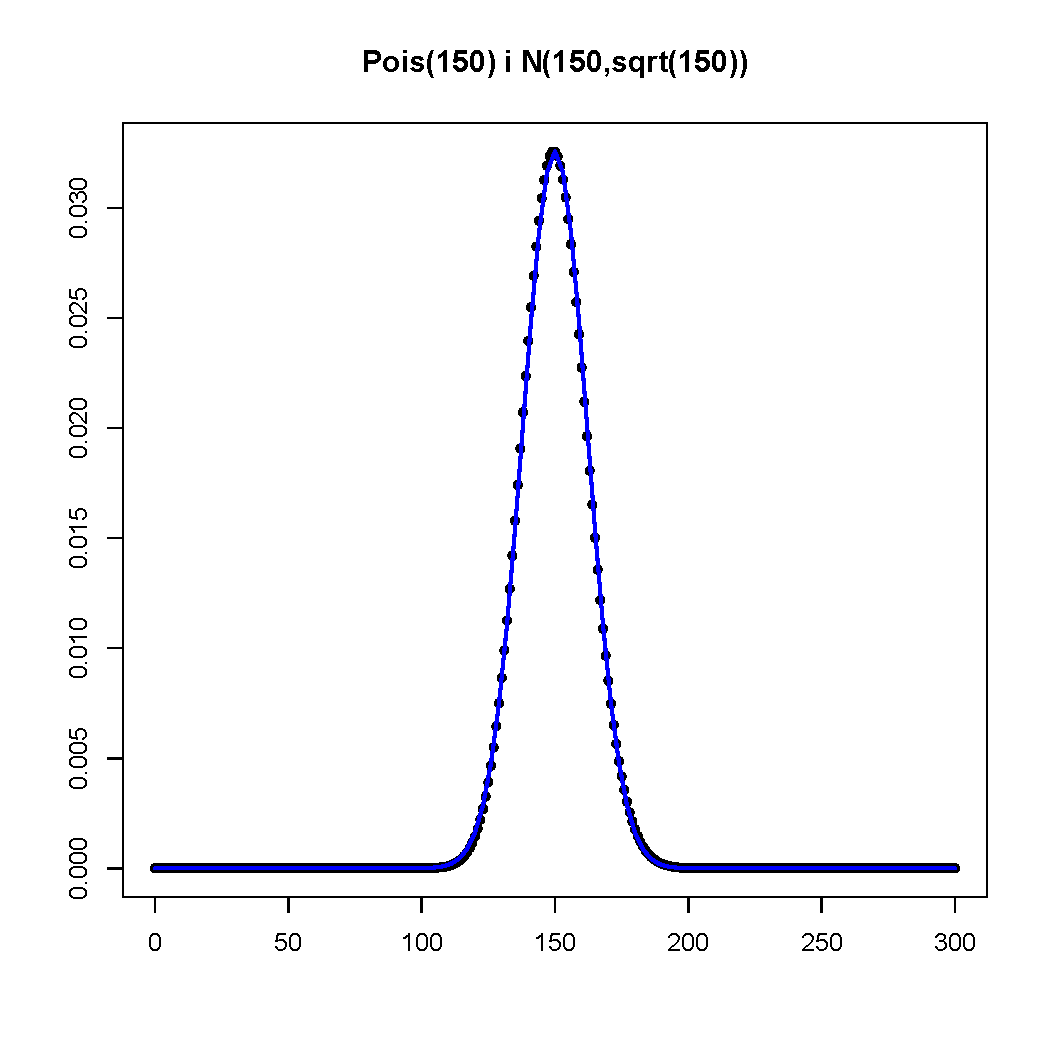
\includegraphics[width=0.6\linewidth]{poisvsnormal1}
% \end{center}
% \vspace*{-1cm}

\begin{knitrout}
\definecolor{shadecolor}{rgb}{0.969, 0.969, 0.969}\color{fgcolor}
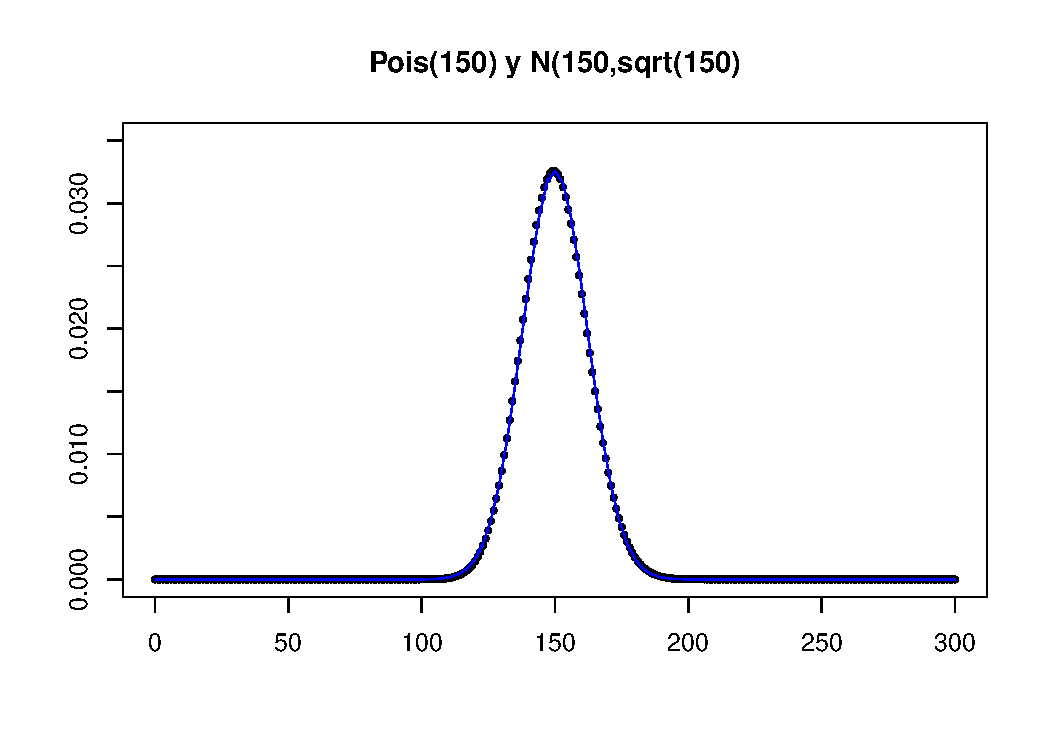
\includegraphics[width=\maxwidth]{figure/unnamed-chunk-6-1} 

\end{knitrout}



Esta aproximación no es tan buena como con las binomiales.
\end{frame}


\begin{frame}



\frametitle{(OPCIONAL)Aproximación de una Poisson por una normal}


\begin{teorema}
Sea  $X$ una v.a. $Po(\lambda)$, con  $\lambda$ grande. Sea $Y$ una v.a. $N(\lambda,\sqrt{\lambda})$ (recordar que $E(X)\!=\!Var(X)\!=\!\lambda$). Entonces 
$$
P(X=k)\approx  P\left(k-0.5\leq Y\leq k+0.5\right)
$$
\end{teorema}
Por lo tanto, si $X$ es una v.a. $Po(\lambda)$ con $\lambda$ grande,
$$
\frac{X-\lambda}{\sqrt{\lambda}}
$$
se aproxima por una normal estándar $Z$, en  el sentido anterior
$$
P(X=k) \approx P\left(\dfrac{k-0.5-\lambda}{\sqrt{\lambda}}
\leq Z \leq \dfrac{k+0.5-\lambda}{\sqrt{\lambda}}\right)
$$

\end{frame}


\end{document}







